\subsubsection{Sistemas Din\'amicos}
\label{sec:SistemasDinamicos}
    La teor\'ia de Sistemas Din\'amicos puede considerarse una forma de describir c\'omo un determinado estado
        se transforma o evoluciona en otro a lo largo del tiempo, es decir, c\'omo evoluciona un sistema en el tiempo.
        La teor\'ia de Sistemas Din\'amicos se puede aplicar a cualquier \'area de la ciencia, como por ejemplo,
        la biolog\'ia, la econom\'ia, la f\'isica, la qu\'imica, etc. En nuestro caso en particular, la teor\'ia de
        Sistemas Din\'amicos se aplica a los aut\'omatas celulares, ya que los aut\'omatas celulares son sistemas
        din\'amicos discretos.
    \vskip 0.5cm
    Nos referimos a sistemas din\'amicos discretos cuando el tiempo es discreto. Con los aut\'omatas celulares
        podemos ver que el tiempo es discreto, ya que el tiempo se mide en generaciones. Es decir, en cada generaci\'on
        el aut\'omata celular evoluciona de un estado a otro. En la Figura \ref{fig:automataCelularEvolucion} podemos
        ver un ejemplo de la evoluci\'on de un aut\'omata celular en el tiempo:
        \begin{figure}[h]
            \centering
            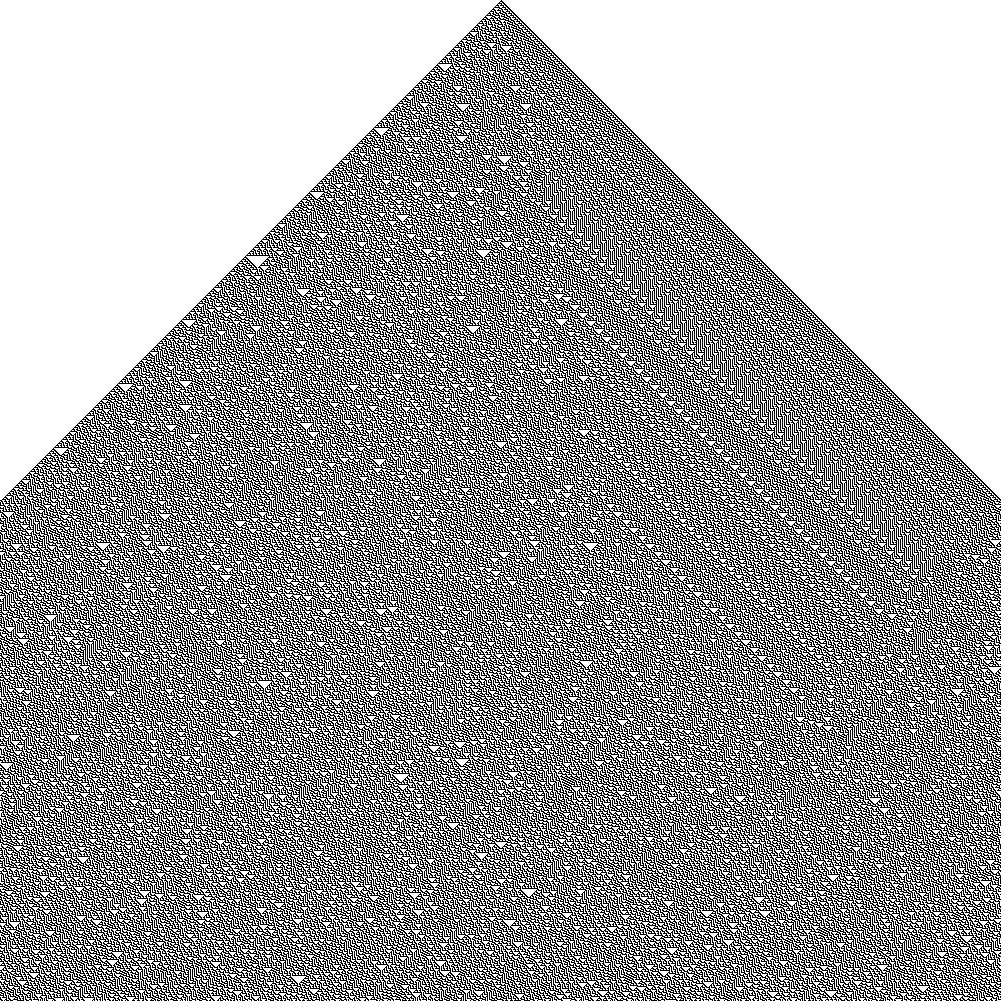
\includegraphics[width=0.5\textwidth]{./images/marco_teorico/automatas_celulares/Regla30-1000Gen.png}
            \caption{Evoluci\'on de la regla 30 en 1000 generaciones o pasos de tiempo}
            \label{fig:automataCelularEvolucion}
        \end{figure}
    \vskip 0.5cm
    No daremos una explicaci\'on m\'as en profundidad de los sistemas din\'amicos, ya que no es el objetivo de este
        trabajo. Para m\'as informaci\'on sobre sistemas din\'amicos y caos, se recomienda leer \cite{Ott1993} y tambi\'en \cite{Luenberger1979}.
        Sin embargo, lo que s\'i es importante mencionar es que los sistemas din\'amicos pueden ser clasificados,
        en este caso nos enfocaremos en los sistemas triviales, los sistemas complejos y los sistemas ca\'oticos.
    \vskip 0.5cm
    Esto lo hacemos con el prop\'osito de poder clasificar el comportamiento de nuestro aut\'omata celular (Physarum Polycephalum)
        en base a su comportamiento. Es decir, si el aut\'omata celular se comporta de manera trivial, compleja o ca\'otica.
        Para esto, primero daremos una breve explicaci\'on de cada uno de estos tipos de sistemas din\'amicos. A su vez, 
        quisi\'eramos destacar que para hacer nuestra clasificaci\'on o determinar el tipo de comportamiento tiene nuestro aut\'omata
        celular usaremos una gr\'afica en la cual podamos observar la Entrop\'ia de Shannon en funci\'on del tiempo. Ya que para
        poder usar como m\'etodo de clasificaci\'on los atractores, requerimos que la cantidad de estados en el Physarum Polycephalum
        es: $\mathbb{P} = \{x \in \mathbb{Z}| 0 \leq x \leq 8\}$ entonces es $S = \mathbb{P}$ y por lo tanto su funci\'on de transici\'on es: 
        $f: \mathbb{P} \rightarrow \mathbb{P}$ o sea $f: \mathbb{P}^{N} \rightarrow \mathbb{P}$ donde $N$ es la vecindad del aut\'omata celular.
        Por lo tanto, la funci\'on de transici\'on es una funci\'on de $\mathbb{P}^{9}$, 
        dandonos como resultado un total de $9^{9}$ o sea 387,420,489 estados posibles. Por lo tanto, no es posible graficar todos los
        estados posibles del aut\'omata celular.
    \vskip 0.5cm
    Ahora si, daremos una breve explicaci\'on de los sistemas mencionados anteriormente:
    \begin{itemize}
        \item \textbf{Sistemas Triviales:} Son sistemas que no tienen comportamiento complejo, es decir, son sistemas que
            tienen un comportamiento predecible. Por ejemplo, un p\'endulo simple, ya que su movimiento es peri\'odico y predecible.
        \item \textbf{Sistemas Complejos:} Son sistemas que tienen un comportamiento complejo, es decir, son sistemas que
            tienen un comportamiento impredecible debido a su sensibilidad a las condiciones iniciales y a la presencia de interacciones no 
            lineales.  Por ejemplo, el clima, ya que es imposible predecir el clima con exactitud.
        \item \textbf{Sistemas Ca\'oticos:} Los sistemas ca\'oticos son un subconjunto de sistemas complejos que son extremadamente sensibles 
            a las condiciones iniciales. Peque\~nas variaciones en las condiciones iniciales pueden llevar a resultados completamente diferentes en el
            tiempo. Los sistemas ca\'oticos pueden parecer aleatorios y desordenados, pero en realidad est\'an gobernados por ecuaciones matem\'aticas 
            deterministas. Un ejemplo cl\'asico de sistema ca\'otico es el sistema de doble p\'endulo, donde el movimiento se vuelve impredecible y 
            altamente sensible a las condiciones iniciales despu\'es de un corto per\'iodo de tiempo.
    \end{itemize}
